\section{Question 1}
\textit{Estimate the natural frequency of the system by determining the motor frequency that results in the largest measured displacement amplitude.}

From the dataset Table \ref{tab:frequency_response} in Section \ref{sec:sample_calculations}, the largest measured displacement amplitude was 0.00198m, which occurs at a motor frequency of $\boxed{5.23 \text{Hz}}$.

\section{Question 2}
\textit{Plot $\mathbb{X}$ vs. $\omega/p$ to obtain the frequency response curve of the system.}
The data from Table \ref{tab:frequency_response} was plotted using Matplotlib in Python \cite{matplotlib}. The plot is shown in Figure \ref{fig:frequency_response_curve}. 
\begin{figure}[H]
    \centering
    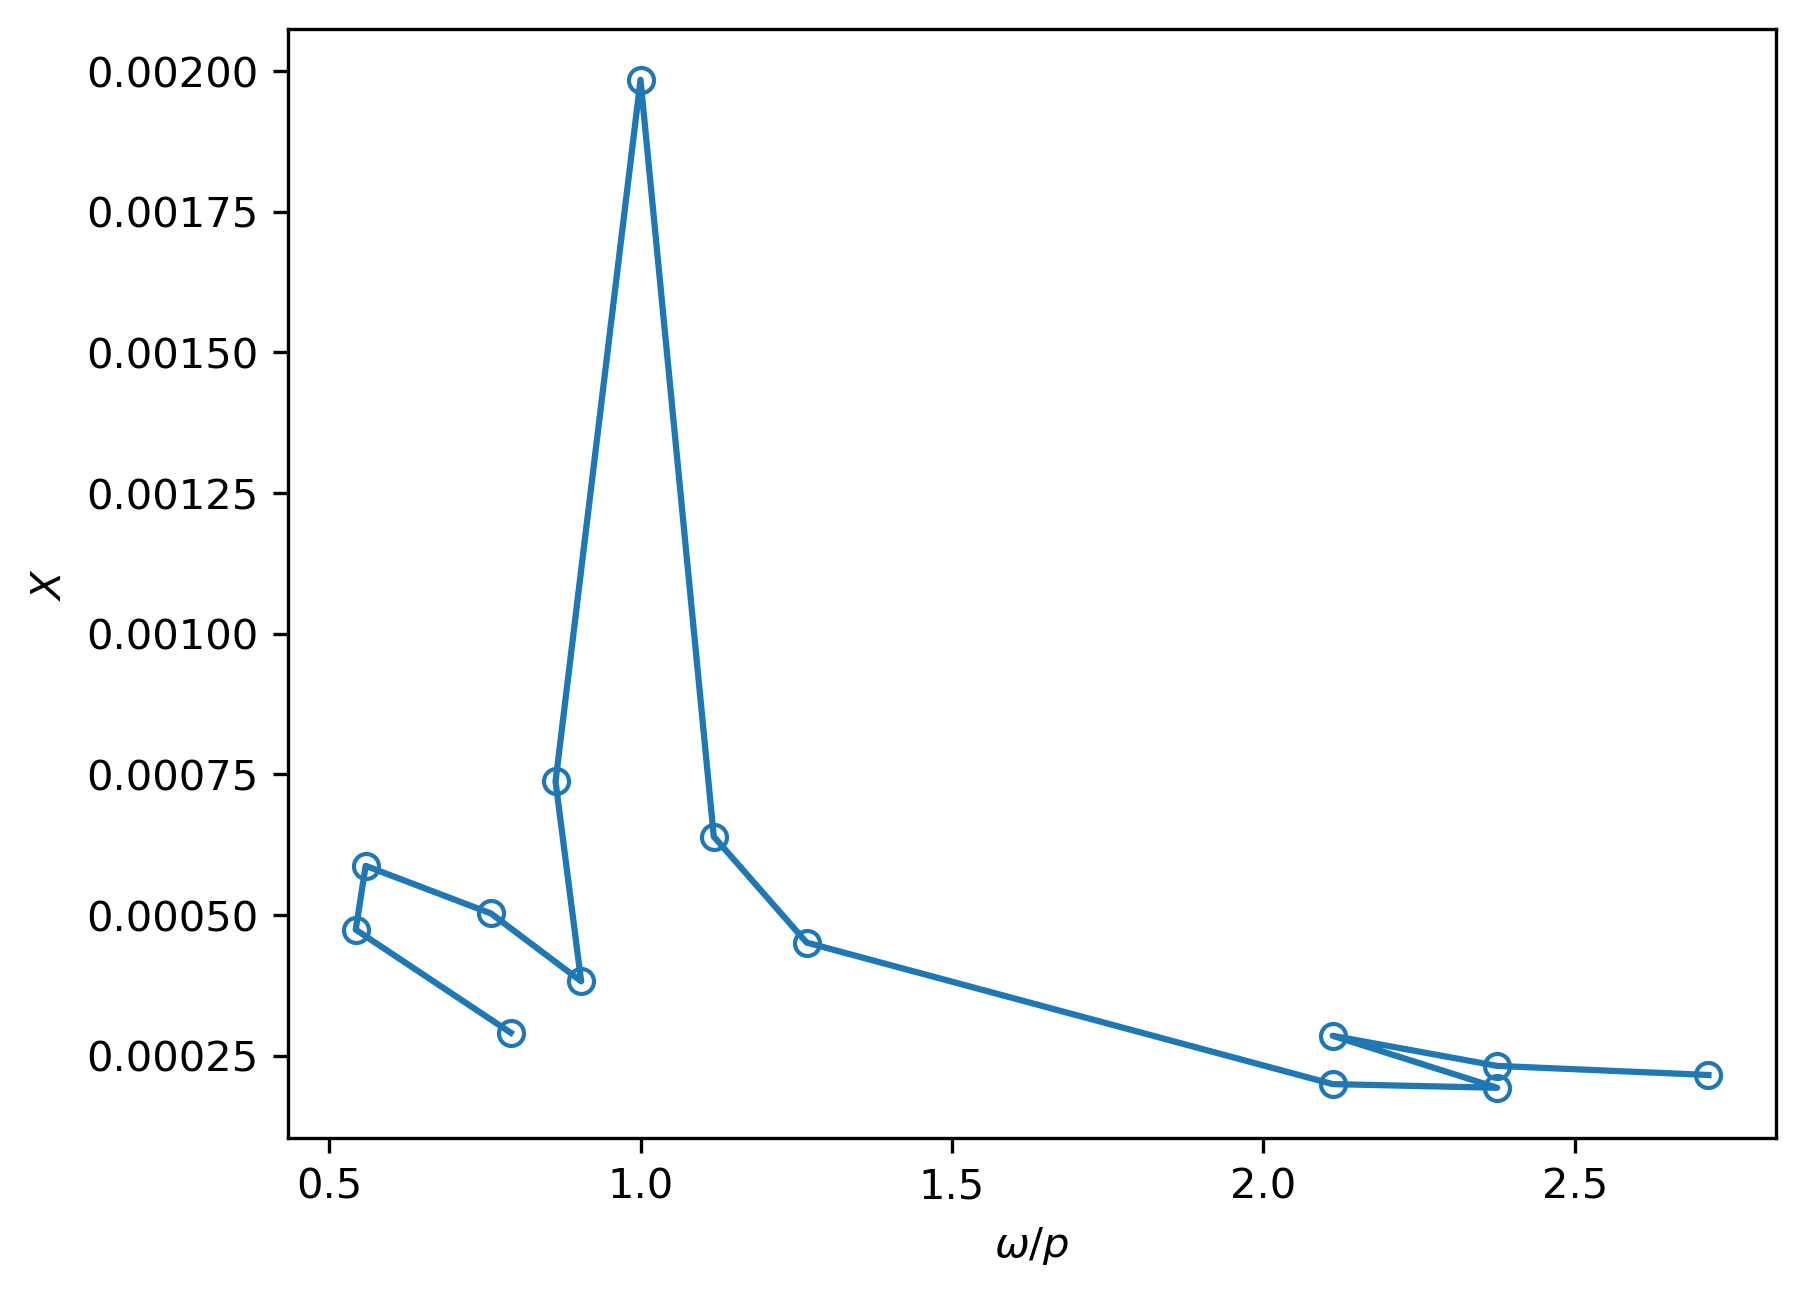
\includegraphics[width=0.8\textwidth]{Questions/Plots/X_vs_omega_p.png}
    \caption{Amplitude vs. $\omega/p$ Response Curve}
    \label{fig:frequency_response_curve}
\end{figure}

\section{Question 3}
\textit{Using your plot of $\mathbb{X}$ vs. $\omega/p$, estimate the damping ratio using the half-power bandwidth method. $\omega_1$ and $\omega_2$ can be determined using linear interpolation.}
\begin{figure}[H]
    \centering
    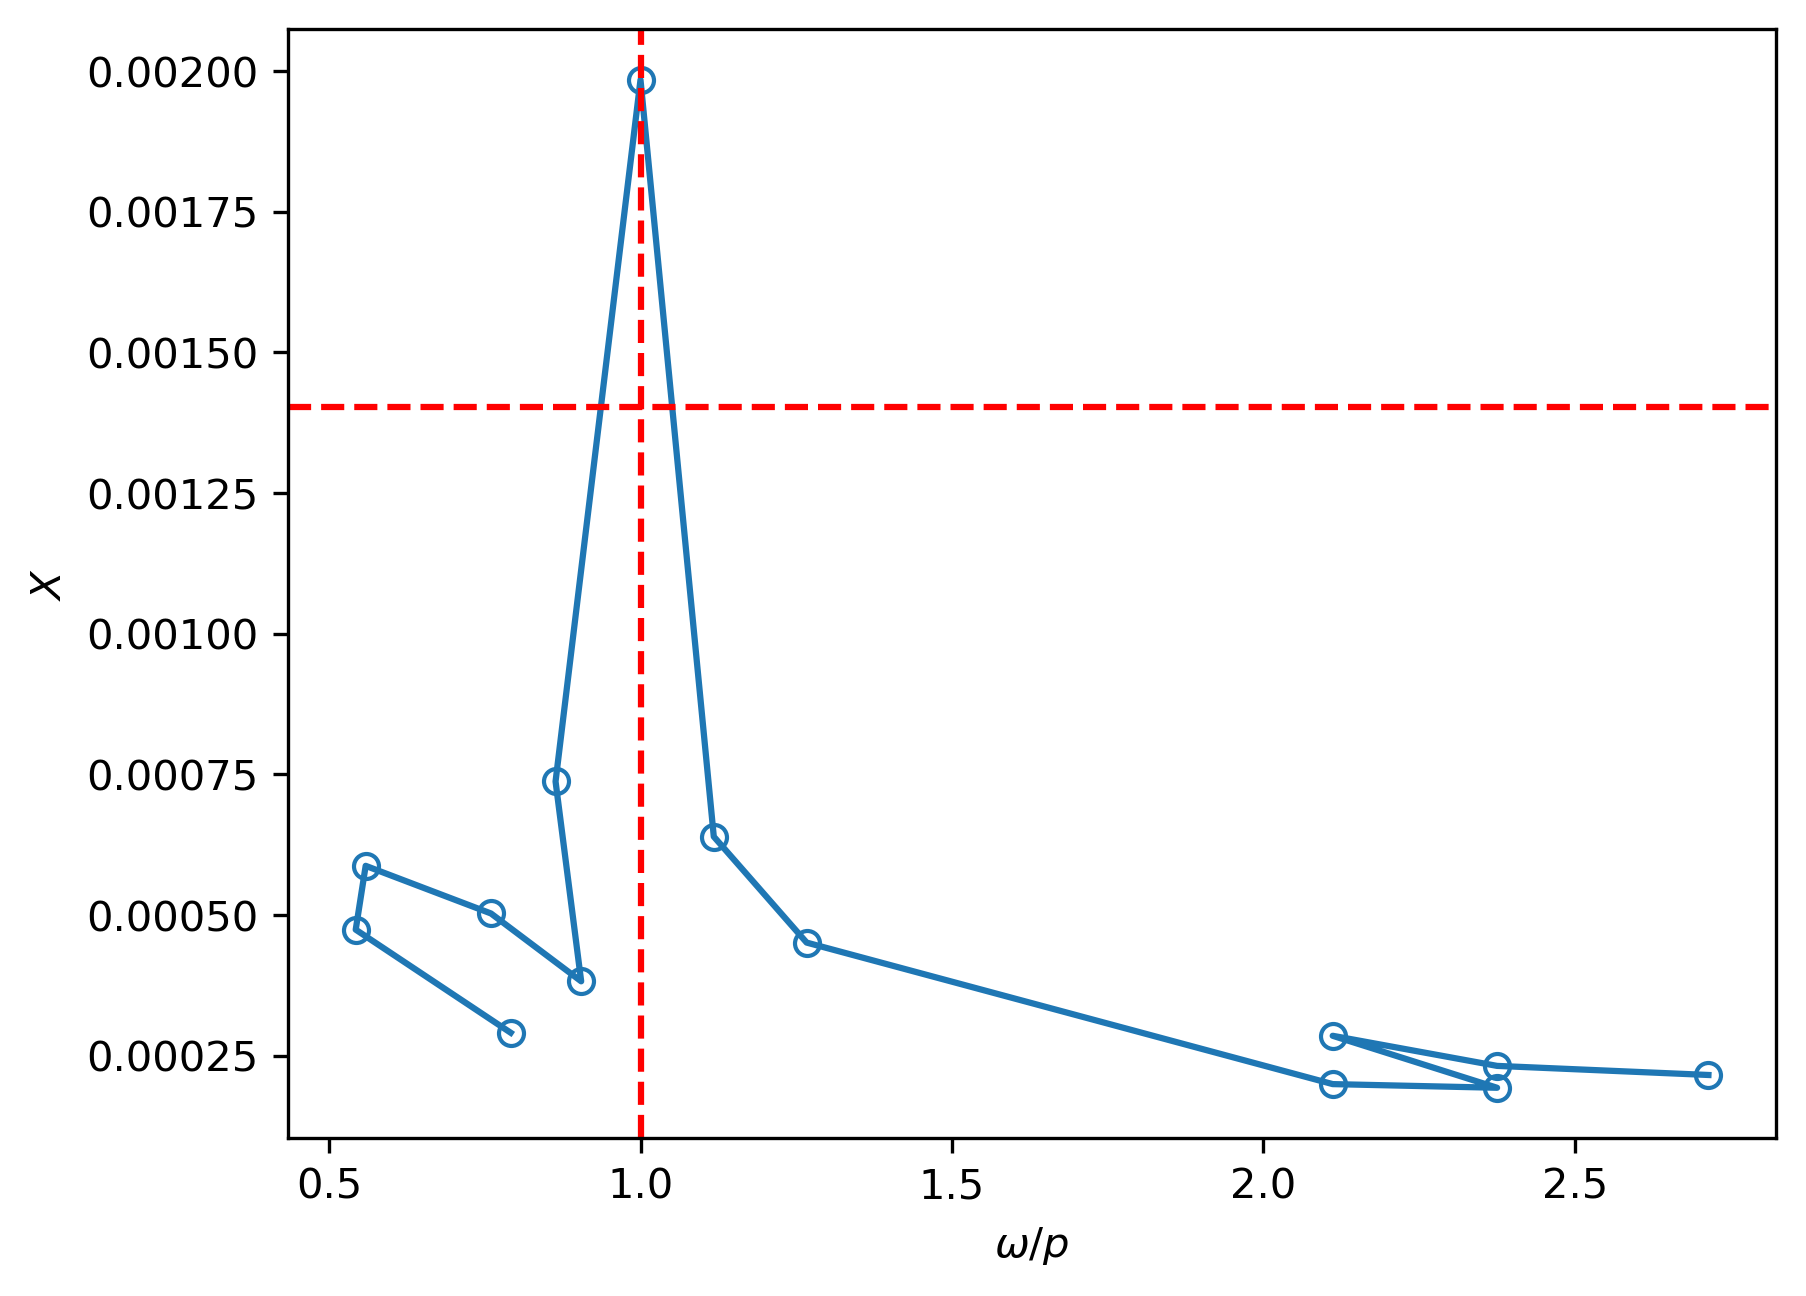
\includegraphics[width=0.8\textwidth]{Questions/Plots/X_vs_omega_p_with_lines.png}
    \caption{Annotated Amplitude vs. $\omega/p$ Response Curve}
    \label{fig:frequency_response_curve_with_lines}
\end{figure}
From the annotated frequency response curve in Figure \ref{fig:frequency_response_curve_with_lines}, the half-power bandwidth method was used to estimate the damping ratio. From linear interpolation of the LHS of the peak, denoting ($x$, $y$) = ($\omega/p$, $\mathbb{X}$), 
\begin{align*}
    x_{\text{LHS}} &= \frac{x_1 - x_2}{y_1 - y_2} \left(\frac{y_1}{\sqrt{2}} - y_1\right) + x_1 \\
    &= \frac{1 - 0.864}{0.00198 - 0.00737} \left(\frac{0.00198}{\sqrt{2}} - 0.00198\right) + 0.00198 \\
    &= 0.9364 
\end{align*}
For the RHS of the peak,
\begin{align*}
    x_{\text{RHS}} &= \frac{x_1 - x_2}{y_1 - y_2} \left(\frac{y_1}{\sqrt{2}} - y_1\right) + x_1 \\
    &= \frac{1 - 0.864}{0.00198 - 0.00639} \left(\frac{0.00198}{\sqrt{2}} - 0.00198\right) + 0.00198 \\
    &= 1.0508
\end{align*}
Then by the half-power bandwidth method, the damping ratio, $\zeta$, was calculated by
\begin{align*}
    \zeta = \frac{\omega_2 - \omega_1}{2p} &= \frac{\omega_{\text{RHS}}/p - \omega_{\text{LHS}}/p}{2} \\
    &= \frac{1.0508 - 0.9364}{2} \\
    &= \boxed{0.0572}
\end{align*}

\section{Question 4}
\textit{Using your calculated damping ratio, estimate the mass of a single imbalance (remember that there are two imbalances, not one), if they each have an eccentricity of 25 mm. Assume the total mass of the system is 13 kg.}

From Eq. (5.22),
\begin{align*}
    \frac{M \mathbb{X}}{\tilde{m}e} &= \frac{\left(\frac{\omega}{p}\right)^2}{\sqrt{\left[1 - \left(\frac{\omega}{p}\right)^2\right]^2 + \left(2\zeta\frac{\omega}{p}\right)^2}} 
\end{align*}
Rearranging,
\begin{align*}
    \tilde{m} &= \frac{M \mathbb{X}}{e} \frac{\sqrt{\left[1 - \left(\frac{\omega}{p}\right)^2\right]^2 + \left(2\zeta\frac{\omega}{p}\right)^2}}{\left(\frac{\omega}{p}\right)^2} 
\end{align*}
Using Dataset \#7 from Table \ref{tab:frequency_response}, 
\begin{align*}
    \tilde{m} &= \frac{13 \times 1.98 \times 10^{-3}}{0.025} \frac{\sqrt{\left[1 - \left(1\right)^2\right]^2 + \left(2 \times 0.0572 \times 1\right)^2}}{\left(1\right)^2} \\
    &= 0.11778624 \text{ kg}
\end{align*}
Since there are two imbalances, the mass of a single imbalance is 
\begin{align*}
    \boxed{m = 0.0589 \text{ kg}}
\end{align*}

\section{Question 5}
\textit{Estimate the natural frequency of the system using the vertical acceleration data recorded during beating of the platform and the motor frequency measured with the stroboscope.}
The beating results are shown in Table \ref{tab:beating_results}. The maximum, minimum, and times were determined by inspection. The frequency was calculated by
\begin{align*}
    f_{\text{Phyphox}} &= \frac{1}{2(t_{\text{min}} - t_{\text{max}})} \\
    &= \frac{1}{2(3.249 - 3.349)} \\
    &= \boxed{4.969 \text{ Hz}}
\end{align*}

The natural frequency was also determined by stroboscope to be 
\begin{align*}
    f_{\text{Stroboscope}} &= \boxed{5 \text{ Hz}}
\end{align*}


\begin{table}[H]
    \centering
    \caption{Beating Results}
    \label{tab:beating_results}
    \begin{tabular}{C{0.10\textwidth}C{0.10\textwidth}C{0.10\textwidth}C{0.10\textwidth}C{0.15\textwidth}C{0.15\textwidth}}
        \toprule
        Max Acceleration, $a_{\text{max}}$ & Min Acceleration, $a_{\text{min}}$ & Time of Max, $t_{\text{max}}$ & Time of Min, $t_{\text{min}}$ & Acceleration Amplitude, $\mathbb{A}$ & Frequency, $f$ \\
        (m/s$^2$) & (m/s$^2$) & (s) & (m/s$^2$) & (Hz) \\
        \midrule
        1.640 & -1.438 & 3.349 & 3.249 & 1.539 & 4.969 \\
        \bottomrule
    \end{tabular}
\end{table}

\section{Sample Calculations}
\label{sec:sample_calculations}
\textit{Use your accelerometer data (in the z direction) to estimate the frequency of the motor $\omega$ and the corresponding displacement amplitude $\mathbb{X}$ of the platform for each motor speed}
\begin{table}[H]
    \centering
    \caption{Frequency and Displacement Results}
    \label{tab:frequency_response}
    \resizebox{\textwidth}{!}{
    \begin{tabular}{C{0.10\textwidth}C{0.10\textwidth}C{0.10\textwidth}C{0.10\textwidth}C{0.10\textwidth}C{0.15\textwidth}C{0.10\textwidth}C{0.10\textwidth}C{0.10\textwidth}C{0.15\textwidth}C{0.10\textwidth}}
        \toprule
        Dataset \# & Max Acceleration, $a_{\text{max}}$ & Min Acceleration, $a_{\text{min}}$ & Time of Max, $t_{\text{max}}$ & Time of Min, $t_{\text{min}}$ & Acceleration Amplitude, $\mathbb{A}$ & Frequency, $f$ & Angular Frequency, $\omega$ & Displacement Amplitude, $\mathbb{X}$ & $\omega/p$ \\
        & (m/s$^2$) & (m/s$^2$) & (s) & (s) & (m/s$^2$) & (Hz) & (rad/s) & (m) & \\
        \midrule
        1 & 0.210 & -0.184 & 5.960 & 6.081 & 0.197 & 4.141 & 26.021 & 2.91E-04 & 0.792 \\
        2 & 0.147 & -0.155 & 7.130 & 7.306 & 0.151 & 2.840 & 17.843 & 4.74E-04 & 0.543 \\
        3 & 0.176 & -0.220 & 12.155 & 12.326 & 0.198 & 2.923 & 18.368 & 5.87E-04 & 0.559 \\
        4 & 0.306 & -0.321 & 16.422 & 16.548 & 0.314 & 3.976 & 24.980 & 5.03E-04 & 0.760 \\
        5 & 0.284 & -0.392 & 20.974 & 21.080 & 0.338 & 4.733 & 29.738 & 3.82E-04 & 0.905 \\
        6 & 0.578 & -0.610 & 28.302 & 28.191 & 0.594 & 4.518 & 28.387 & 7.37E-04 & 0.864 \\
        7 & 2.044 & -2.244 & 35.249 & 35.345 & 2.144 & \textbf{5.231} & 32.869 & 1.98E-03 & 1.000 \\
        8 & 0.897 & -0.828 & 43.280 & 43.194 & 0.863 & 5.847 & 36.736 & 6.39E-04 & 1.118 \\
        9 & 0.854 & -0.710 & 52.083 & 52.008 & 0.782 & 6.626 & 41.634 & 4.51E-04 & 1.267 \\
        10 & 1.019 & -0.901 & 58.312 & 58.267 & 0.960 & 11.044 & 69.389 & 1.99E-04 & 2.111 \\
        11 & 1.282 & -1.068 & 64.397 & 64.357 & 1.175 & 12.424 & 78.063 & 1.93E-04 & 2.375 \\
        12 & 1.385 & -1.362 & 69.977 & 69.932 & 1.373 & 11.044 & 69.389 & 2.85E-04 & 2.111 \\
        13 & 1.629 & -1.195 & 74.560 & 74.520 & 1.412 & 12.424 & 78.063 & 2.32E-04 & 2.375 \\
        14 & 1.896 & -1.536 & 86.093 & 86.057 & 1.716 & 14.199 & 89.215 & 2.16E-04 & 2.714 \\
        \bottomrule
    \end{tabular}
    }
\end{table}
Sample calculations will be shown for dataset \#1. From the data, $a_{\text{max}}$, $a_{\text{min}}$, $t_{\text{max}}$, and $t_{\text{min}}$ were determined by inspection. Then, the amplitude of the acceleration, $\mathbb{A}$, was calculated by
\begin{equation*}
    \mathbb{A} = \frac{a_{\text{max}} - a_{\text{min}}}{2} = \frac{0.210 - (-0.184)}{2} = 0.197 \text{ m/s}^2
\end{equation*}
The frequency, $f$, was calculated by
\begin{equation*}
    f = \frac{1}{2(t_{\text{min}} - t_{\text{max}})} = \frac{1}{2(6.081 - 5.960)} = 4.141 \text{ Hz}
\end{equation*}
The angular frequency, $\omega$, was calculated by
\begin{equation*}
    \omega = 2\pi f = 2\pi(4.141) = 26.021 \text{ rad/s}
\end{equation*}
The displacement amplitude, $\mathbb{X}$, was calculated by
\begin{equation*}
    \mathbb{X} = \frac{\mathbb{A}}{\omega^2} = \frac{0.197}{(26.021)^2} = 2.91 \times 10^{-4} \text{ m}
\end{equation*}
The ratio of the angular frequency to the natural frequency, $\omega/p$, was calculated by
\begin{equation*}
    \omega/p = \frac{\omega}{p} = \frac{26.021}{33} = 0.792
\end{equation*}

